\newpage

\section*{ $^{27}$Al(n,$\alpha$)$^{24}$Na }

Power Level: 100 kW(th) \\
Time at Power: 60.0 m \\
Wait Time:  2.0 d \\
Counting Time: 60.0 m \\
Total Activity at Removal: 2.80e-01 $\mu Ci$

\begin{table*}[h]
\centering
\begin{tabular}{ |c|c|c|c|c|c| }
 \hline
 Position & Mass $mg$ & Counting Activity $\mu Ci$ & Area (Counts) & Error \% \\
 \hline 
 1 & 3.50 & 7.53e-03 & 1.47e+04 & 0.8245 \\ 
\hline
 2 & 3.50 & 1.10e-02 & 2.14e+04 & 0.6829 \\ 
\hline
 3 & 3.50 & 8.10e-03 & 1.58e+04 & 0.7949 \\ 
\hline
 4 & 3.50 & 3.60e-03 & 7.04e+03 & 1.1920 \\ 
\hline
\end{tabular}
\end{table*}

\begin{figure}[h]
\centering
\begin{subfigure}{.5\textwidth}
  \centering
     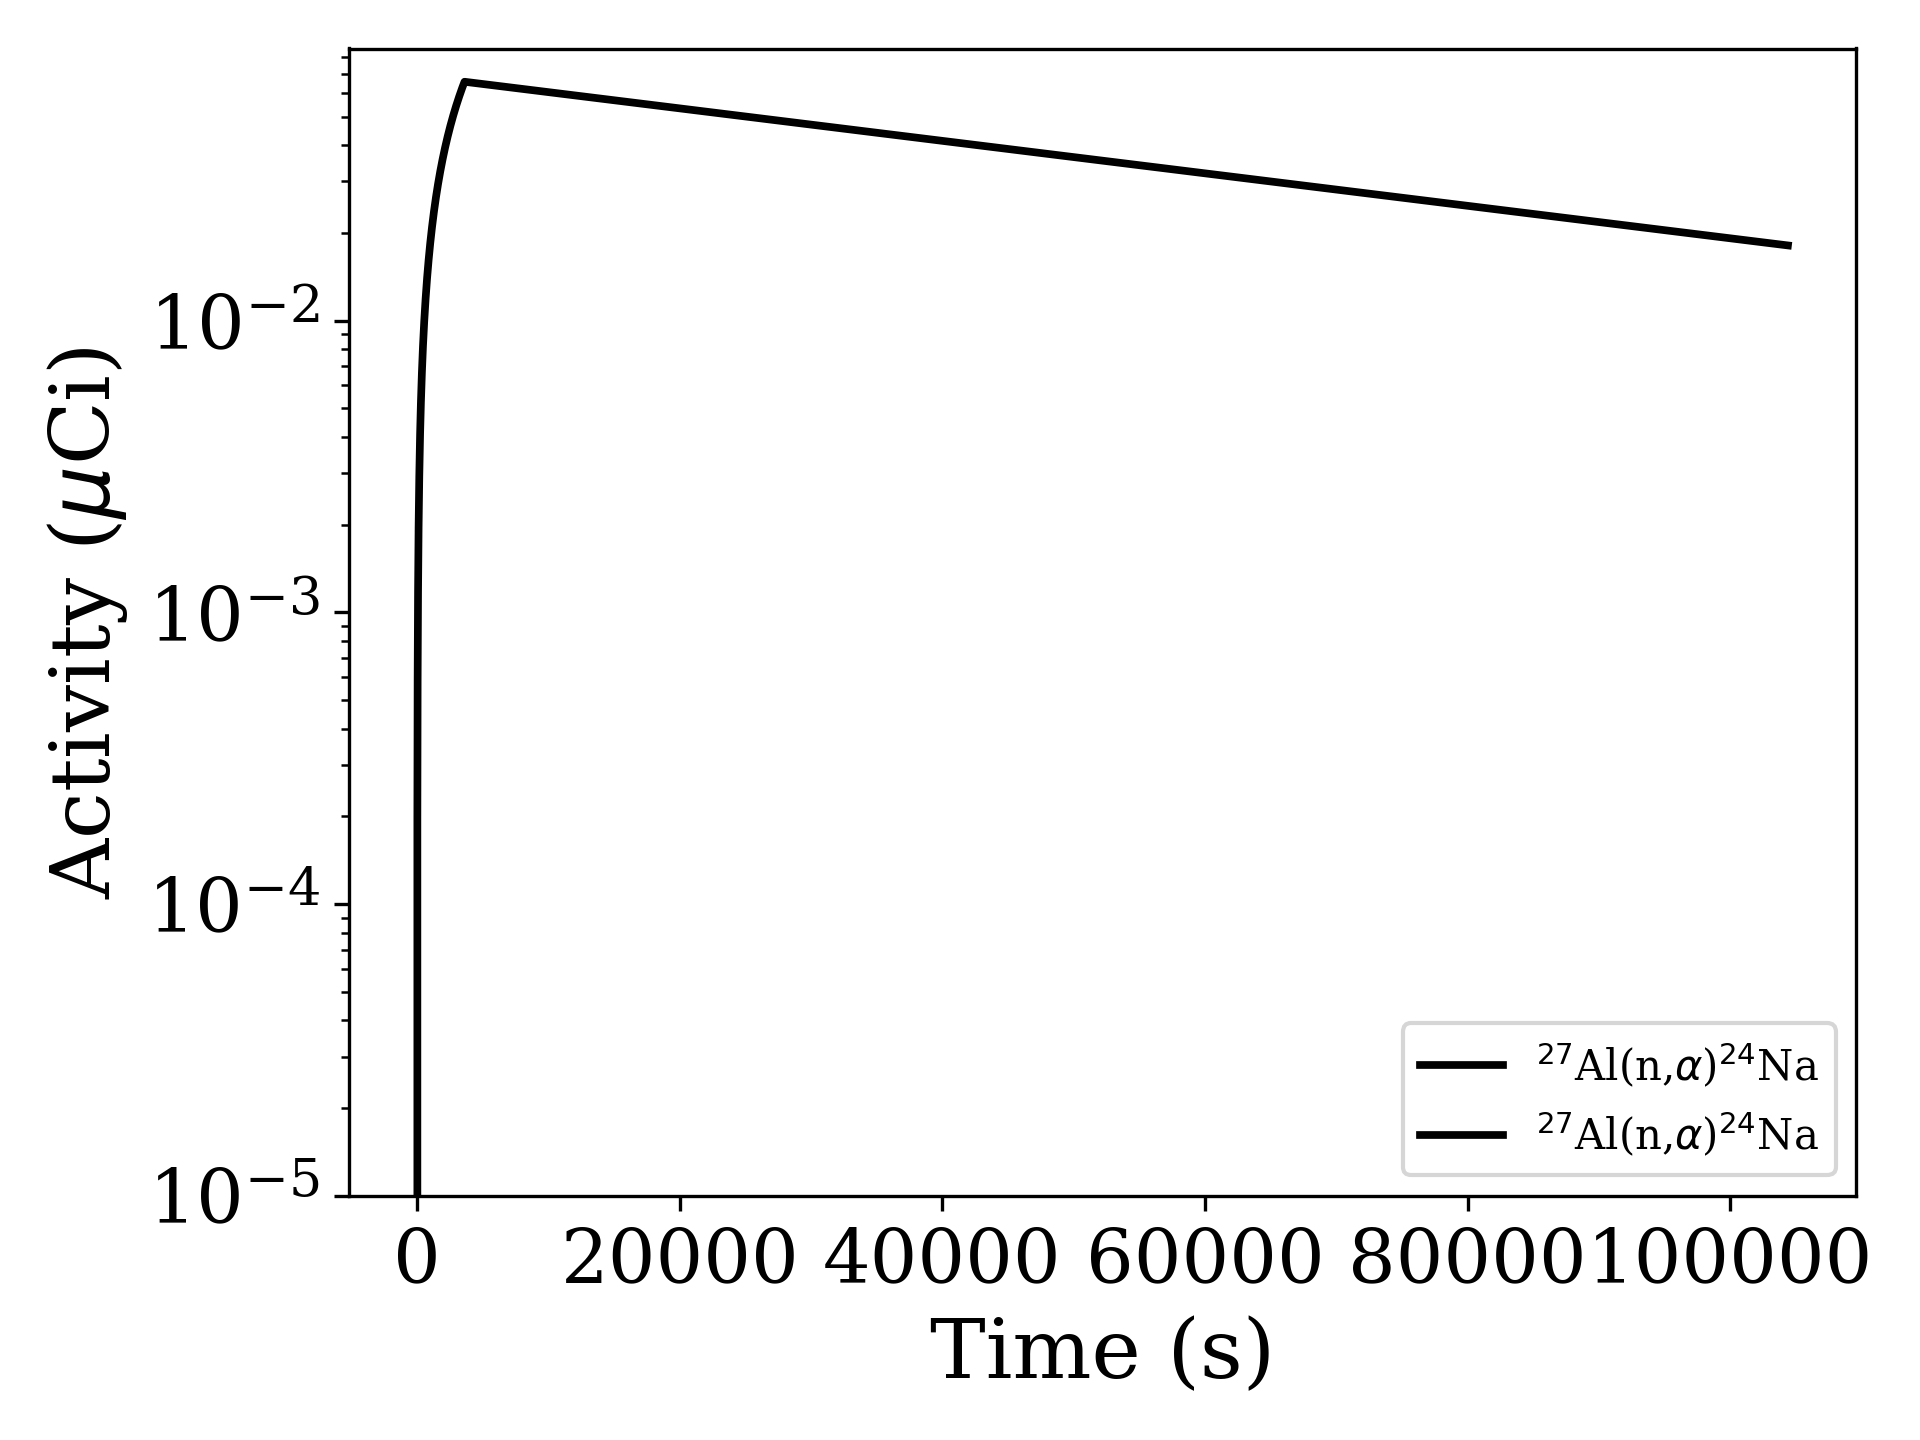
\includegraphics[width=.8\textwidth]{plot/Al-27(n,alpha)Na-24_wisconsin1} 

  \caption{Activity}
\end{subfigure}%
\begin{subfigure}{.5\textwidth}
  \centering
     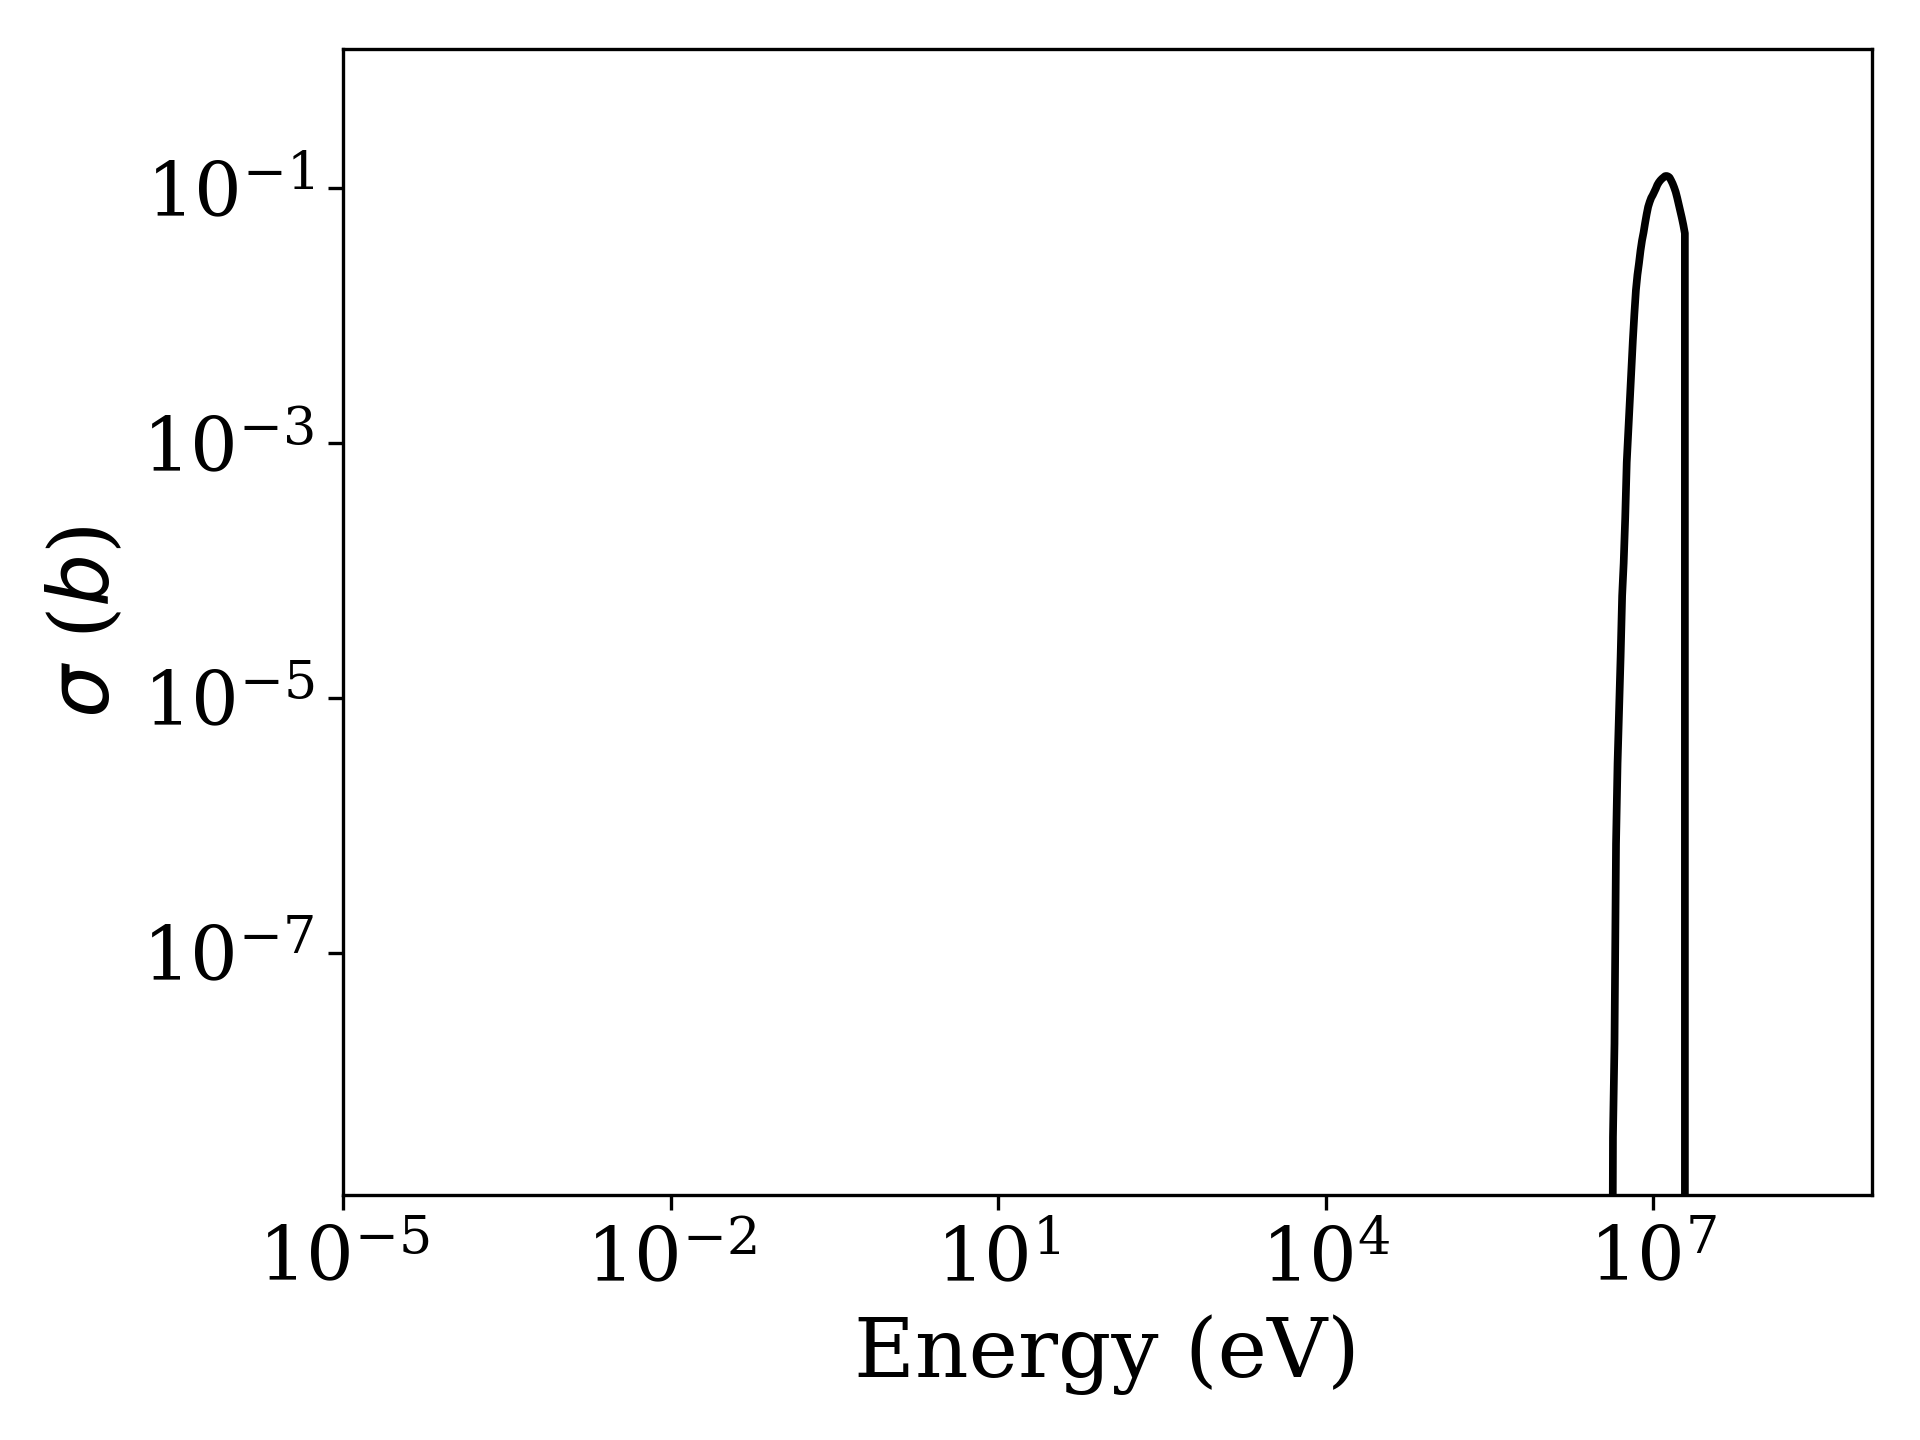
\includegraphics[width=.8\textwidth]{plot/Al-27(n,alpha)Na-24} 

  \caption{Cross Section}
\end{subfigure}
\end{figure}

\begin{table*}[h]
\centering
\begin{tabular}{ |c|c|c|c|c|c|c| }
 \hline
 Reaction & T$_{1/2}$ & ROI (eV) & Important Gammas (keV) \\
 \hline 
 $^{27}$Al(n,$\alpha$)$^{24}$Na & 15.0 h & 6.56e+06, 1.21e+07 & 1368.626(0.999936) \\ 
\hline
\end{tabular}
\end{table*}
